\documentclass[final]{siamltex}

\usepackage{cite}
\usepackage{multirow}
\usepackage{graphicx}
\usepackage{url}

% correct bad hyphenation here
\hyphenation{}

\usepackage{xspace}

\def\gled{\textsc{Gled}\xspace}
\def\p7{\textsc{Project7}\xspace}
\def\grid{\texttt{grid}\xspace}
\def\smalltt#1{{\small\texttt{#1}}}
\def\foottt#1{{\footnotesize\texttt{#1}}}

%\looseness=-1 end slimy pars with this

\title{\gled\ -- an Implementation of a Hierarchic Server--Client Model}


\author{Matev\v{z} Tadel\thanks{``Jo\v{z}ef Stefan Institute'', Jamova 39,
    SI-1000 Ljubljana,
    Slovenia ({\tt Matevz.Tadel@ijs.si})}}

\begin{document}

\maketitle

\begin{abstract}
  \gled is an implementation of a hierarchic server--client model
  written in \smalltt{C++}, having an outside form of an object
  oriented framework. Master server exposes its object space to its
  first-level clients which in turn provide mirroring facilities to
  second-level clients and also export their own object spaces. Each
  client therefore plays a role of a client, a proxy and a server.
  Infrastructure for propagation and broadcasting of method invocation
  requests is provided and is general enough to allow for an efficient
  access control. Synchronization of object spaces is achieved via
  streaming of object graphs and a time-ordered delivery of method
  invocation requests.
%
  Objects can acquire their own threads to perform different tasks
  such as computation, data acquisition \& analysis or dynamic
  visualization. The obtained results can be pushed to other computing
  nodes or storage devices. As threads are spawned and controlled
  by standard method invocation requests, schedulers \& job control
  mechanisms spawning across a whole \gled cluster can easily be
  implemented.
%
  On viewer level, \gled features automatically generated GUI widgets
  and a sophisticated 3D rendering infrastructure.
\end{abstract}

\begin{keywords} 
  hierarchic server-client model for clusters,
  distributed computing,
  object-oriented framework/toolkit,
  remote procedure call implementation,
  data visualization \& presentation
\end{keywords}

\pagestyle{myheadings}
\thispagestyle{plain}
\markboth{M. TADEL}
{\textsc{Gled} -- an Implementation of a Hierarchic Server--Client Model}

%%%%%%%%%%%%%%%%%%%%%%%%%%%%%%%%%%%%%%%%%%%%%%%%%%%%%%%%%%%%%%%%%%%%%%%%
\section{Introduction}
%%%%%%%%%%%%%%%%%%%%%%%%%%%%%%%%%%%%%%%%%%%%%%%%%%%%%%%%%%%%%%%%%%%%%%%%

The basic ideas of \gled are stemming from recent developments in high
energy physics (HEP) computing as well as from modern information
technologies (\texttt{web} \& \texttt{grid}) and concepts of
cyberspace (interactive computer graphics, virtual reality, multi-user
online games). During the last ten years the paradigm of object oriented
programming was making its way into HEP, both by migration of
experiments from \smalltt{fortran} to \smalltt{C++} and appearance of
ROOT data analysis framework \cite{root}. The methodology of a typical
physical analysis didn't change much though: it still consists of
preparing the input, running the batch job(s) and post-processing \&
visualization of output. While ROOT simplifies transfer of data from
batch job processing to analysis framework, the problem of unification
of all the stages of analysis remains only partially addressed and
requires, for its efficient solution, high computing skills on the
part of a user. This is not a serious problem for a large, mature
analysis which takes several days to complete but in early stages of
analysis preparation users typically run many small jobs and thus
aspire for a fast response of computing infrastructure with the least
possible involvement in technicalities.

With the appearance of relatively cheap super-computers in form of
computing clusters and powerful desktop computers the time spent 
maintaining the working environment is contrasted out far more than
ever before. Large computing farms with modern schedulers can easily
handle jobs with minimal time requirements to provide an unhindered
analysis \& algorithm prototyping while desktop computers can store
data in an order of $\sim$100Mb (as well as obtain it via its network
connection) and provide enough computing power for its processing and
visualization. One of the basic aims of the \gled project is to
address these new possibilities and integrate algorithm development,
input preparation, job execution, data visualization and user-to-user
communication in a common environment.

Another element of modern computing that has likewise grown is the
size of datasets and databases being processed, thus putting a heavy
load on all data transport layers, from networks to permanent storage
devices. For WAN-s and inter-cluster communication the problem has
been effectively addressed with the introduction of \grid
technologies, while LAN-s within large computing clusters with
centralized storage systems are still posing a challenge as many
improvements minimizing the data transfers can be envisioned. A
hierarchic structure of computing nodes interwoven with data storage
and communication nodes seems an obvious solution and it provided one
of the models for hierarchic server--client structure of \gled. By
virtue of the hierarchic structure, the inner computing nodes do not
need a direct WAN access. This architecture might also be of prime
interest for distributed multi-user interactive environments where
hierarchic structure allows for balancing of WAN traffic and local CPU
usage.

\subsection{The main design features of \gled}
%%%%%%%%%%%%%%%%%%%%%%%%%%%%%%%%%%%%%%%%%%%%%%

The \gled project aims at building of an object oriented
framework/toolkit by extending the notion of a \smalltt{C++} class. It
provides the following extensions to the \smalltt{C++} class paradigm:

\begin{enumerate}
\item \textbf{Serialization of objects.} ROOT's infrastructure for
  serialization of objects provides a firm base for storage of objects
  and their transmission over the network.
\item \textbf{Serialization of method calls} allows for a transparent
  implementation of remote method calls with objects acting as the
  natural elements that generate/process the requests.
\item \textbf{Automatic generation of GUI classes}. The auto-generated
  widgets always send serialized method calls to the central message
  processing unit and are therefore decoupled from the actual objects
  they are representing. The GUI classes are a convenient way for
  viewing and editing of objects.
\item \textbf{Rendering classes} coupled with \gled's rendering
  infrastructure provide an alternative representation of objects. It
  can be used to build advanced visualization systems or as a
  flexible method for representing and interacting with large object
  collections.
\end{enumerate}

Furthermore, \gled has a low-level support for object aggregation (lists
and smart pointers) allowing an easy construction of arbitrarily
complex object structures (graphs). The object graphs can be shared across a
cluster with the hierarchic server-client paradigm assuring a consistent
object state and proper method call propagation.\looseness=-1

From architectural point of view \gled is designed as a modular
application with a minimal kernel, providing base classes and
hierarchic server-client code. User classes/code can be imported into
a running kernel by dynamic loading of appropriate shared libraries.

\subsection{Development goals}
%%%%%%%%%%%%%%%%%%%%%%%%%%%%%%

The development of the \gled framework focuses on elements that allow
for fast prototyping and implementation of:

\begin{itemize}
\item \textbf{class libraries} for scientific computation and visualization,
\item \textbf{distributed applications} for scientific computing and
  collaborative object-space access/management,
\item \textbf{intra/inter cluster} communication and
  data-transport \& addressing protocols and
\item \textbf{advanced visualization systems} for single and
  multi-user applications.
\end{itemize}

Object \& method call serialization, hierarchic server-client
architecture and GUI \& data presentation elements of \gled also make
it an interesting platform for projects seeking voluntarily contributed
CPU power for CPU intensive distributed computations (e.g.
SETI@Home\cite{seti} and Folding@Home\cite{folding}). The wide
availability of broadband network access for home PCs is turning them
into powerful computational and data analysis engines, suitable also
for tasks with high demands on network throughput. The hierarchic
server-client model can be effectively used to minimize the network
traffic, provided that the topology of a cluster matches that of a
network.

While the main development goal of \gled is to provide a generic
platform for scientific computing and prototyping of \grid protocols,
many of its features might be of interest to a wider public. In
particular, we see two possibilities for extending \gled in this
direction.
\begin{enumerate}
\item Data-base interfaces coupled with GUI and rendering support of \gled
  would allow for an easy implementation of advanced information
  systems.
\item The hierarchic server-client model, object \& method
  serialization and rendering capabilities make \gled an excellent
  platform for implementation of virtual reality systems. In the
  extreme case \gled could even be used as a multi-player game engine.
\end{enumerate}
Both of these extensions would further enhance \gled for its
main purposes. It is our intention to attract open-source developers
from external communities. Their contribution and wider interest for
the project would also allow for an efficient dissemination of \grid
technologies to a wider public.

%%%%%%%%%%%%%%%%%%%%%%%%%%%%%%%%%%%%%%%%%%%%%%%%%%%%%%%%%%%%%%%%%%%%%%%%
\section{Overview and Terminology}
%%%%%%%%%%%%%%%%%%%%%%%%%%%%%%%%%%%%%%%%%%%%%%%%%%%%%%%%%%%%%%%%%%%%%%%%

The basic elements of \gled are objects, specializations of a class
\smalltt{ZGlass}, exported into a hierarchic server--client system.
The common base class provides services for communication with the
\gled system and, together with the \p7 code-glue generator, enables
its instances to be serialized in a context of an object graph as well
as to send and execute \emph{method invocation requests} (MIR).
Compared to RPC \cite{rpc}, MIRs in \gled represent a distributed RPC
implementation of a ``call/no-wait'' variety with internal rules that
allow for propagation of MIRs through the hierarchy of a \gled
cluster. ROOT's streaming mechanism guarantees interoperability of
architectures and in this context corresponds to external data
representation standard (XDR \cite{xdr}) of RPC.

\gled objects are memory-resident and optimised for fast modification
and immediate replication. Nodes in a \gled cluster share data and
collectively modify it. If a given node desires access to some data it
has to mirror it first and after that it receives and sends MIRs to
keep the data in synchronization with the server. This is quite unlike
LDAP \cite{ldap} which is optimised for massive concurrent queries
with slow modification and lazy replication. On the other hand, \gled
objects can be imported from databases, either as static data, as
query results or as dynamic data that can be changed and possibly
reinserted into the database.

To be able to explain the details of functioning and habitat of \gled
objects, an overview of the hierarchic server--client architecture and
basic properties of the \gled system will first be made.


\subsection{Towards a Hierarchic Server--Client Model}
%%%%%%%%%%%%%%%%%%%%%%%%%%%%%%%%%%%%%%%%%%%%%%%%%%%%%%%%%%%%%%%%%%%%%%%%

The basic idea of a hierarchic server-client model lies in extension
of a simple server--client communication graph to a more general tree
structure (Fig.\,\ref{fig:hscm}). The most notable difference, beyond
the appearance of multiple levels, is that each client becomes also a
server for its clients and a proxy in respect to its server (as well
as for all higher servers on the way to the master server). Separation
of server spaces of clients belonging to one server is in fact the
feature that makes the hierarchical model interesting: it allows nodes
to share data selectively, making it visible only to the nodes that
need access to it. The topology of a tree is arbitrary and can change
dynamically. In practice it is dictated by the structure of the
problem being addressed and should provide optimal functioning of the
nodes while minimizing data transfers among different levels of the
cluster hierarchy.

\begin{figure}
\centering
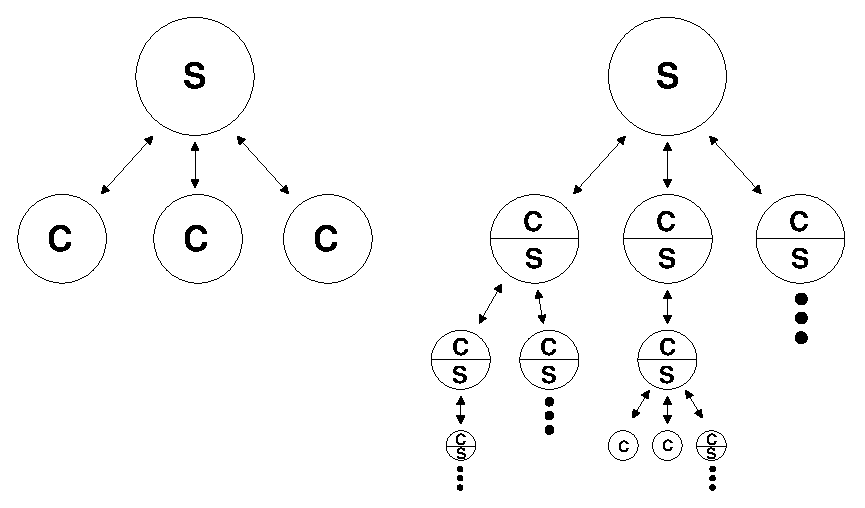
\includegraphics[height=4.45cm]{figs/hscm.eps}
\caption{Comparison of standard (left) and hierarchic (right)
  server--client model. Circles represent computer nodes, while
  labels \textbf{S} and \textbf{C} stand for \emph{server} and
  \emph{client} respectively.}
\label{fig:hscm}
\end{figure}

Another point to notice from the above figure is that a master server
and pure-client nodes are just degenerate cases of the general node
behaviour. This presents a drastic departure from the standard
server-client model. To emphasize this difference and to avoid
confusion, the term \emph{Saturn} was chosen to signify an operational
node in a \gled cluster. The naming is based on the analogy with
planetary system and propagation of light: light emitted by the planet
Saturn is partially the reflected light from the Sun and the rest is
produced by the processes proceeding under the veil of the planet's
atmosphere. The master server is called either a \emph{zeroth-level
 Saturn} or \emph{Sun Absolute}. Additionally, symbol ${\cal S}$ is
used for any Saturn, ${\cal S}_0$ for the Sun Absolute and ${\cal
 S}_i$, $i > 0$ for an \emph{i-th level} Saturn.

Since objects need to be uniquely identified across different nodes,
they are numbered with positive integers spawning an \emph{object ID
 space}. Intervals from the available set are claimed by Saturns in
succession as they get attached into the system.
Fig.\,\ref{fig:ID_space} shows an example of object space partitioning
for a chain of three Saturns. The linear partitioning with
pre-reservation of desired ID-space interval minimizes efforts
associated with routing of MIRs without the loss of generality.

\begin{figure}
\centering
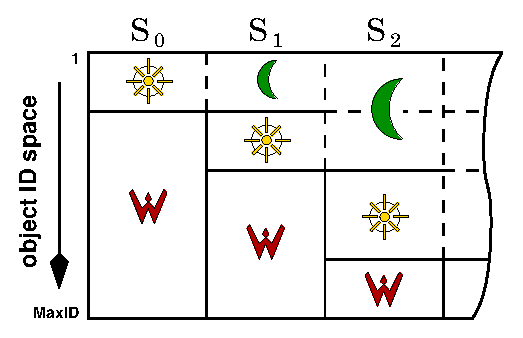
\includegraphics[height=4.5cm]{figs/ID_space.eps}
\caption{A scheme of object ID space partitioning. For each
  Saturn the sun symbol represents its server space, the moon symbol
  its proxy-client space and the fire symbol shows the local space of
  the Saturn.}
\label{fig:ID_space}
\end{figure}

Objects in the server space (or \emph{sun-space}) of ${\cal S}_0$ can
be seen on all \gled nodes. MIRs directed at them from lower Saturns
(or \emph{moons}) are always routed up to ${\cal S}_0$ where the
requests are checked and, if they are accepted, executed and
broadcasted to ${\cal S}_1$ Saturns. They in turn execute the MIR and
broadcast it further down the hierarchy. For a ${\cal S}_i$ Saturn,
the object spaces of all higher Saturns are effectively merged into a
common ID-space partition, called its \emph{moon-space}, providing the
proxy service. This furthers the light analogy: the light emitted by
a Saturn on behalf of its higher Saturns is the reflected light, just
as we see the Moon in the reflected light of our Sun. A Saturn has no
executive power over its moon-space although operations (threads)
issuing from it can perform tasks on behalf of other Saturns.

The same holds for each Saturn: it is the master of its sun-space and
all MIRs affecting it must pass through its execution control prior to
their execution and broadcasting.

Sun-space of each Saturn is further subdivided to allow for its
partial exposure to lower Saturns. Migration of objects between
different object-spaces is also possible. This features are discussed
in section \ref{sec:saturn_os_management}.

Another important feature of such partitioning is the natural arising
of a \emph{local object space} (or \emph{fire-space}) on each Saturn
(Fig.\,\ref{fig:ID_space}). It contains objects pertaining to local
computation and viewing. Fire-space extends over the object-space
following the Saturn's reserved sun-space. As the names suggest,
objects belonging to fire-space are entirely local (light emitted by a
simple fire can not reach other planets). Since global and local
objects share the same ID-space, local objects can easily
reference the global ones to modify their own behaviour. Also, a
user is provided with the same interface in both cases.


\subsection{The Main Aspects of \gled}
%%%%%%%%%%%%%%%%%%%%%%%%%%%%%%%%%%%%%%%%%%%%%%%%%%%%%%%%%%%%%%%%%%%%%%%%

\gled is built upon ROOT \cite{root} and thus inherits its versatile
I/O infrastructure (access of local and remote files with inner
directory structure) and a rich set of data storage, analysis and
presentation functions. CINT \cite{cint}, a C/C++ interpreter, is also
a part of ROOT's heritage and presently plays the role of a scripting
language.\footnote{Currently CINT is not thread safe and therefore
  limits \gled's performance to a single scripting environment per
  Saturn. Usage of a loosely coupled scripting language (e.g.
  \foottt{perl6}) would allow several concurrent scripting sessions.}

As mentioned before, \gled-enabled classes stem from the common base
\smalltt{ZGlass}. Following the analogy with light any \gled class can be
referred to as a \emph{glass} (material, not a vessel) and any
instance as a \emph{lens}. Infrastructure enabling lenses to be fully
operational is rather elaborate and could as such pose a heavy load on
a programmer. To bypass this obstacle, definitions of glasses are
preprocessed by two parsers/code generators:
\begin{itemize}
\item ROOTCINT (part of the ROOT system) produces
  a dictionary, serialization method and interpreter bindings;
\item \p7 (part of \gled) generates accessor methods, methods for
  streaming and processing of MIRs, connectivity introspection methods
  as well as GUI components for a given glass.
\end{itemize}
Both produce code that is in part included back into the class
definition. Therefore some of the class semantics is implicit in
data and function member declarations.

MIRs are always enclosed in a \emph{context}, specifying the target
lens, the identity of a caller and all lens-type arguments.
This allows for authorization and dependency checking prior to
complete unfolding of the request and provides a transparent
way for creation of requests originating from a GUI.

To simplify the extension of the \gled system, build process and
component deployment, glasses and their supporting structures are
grouped into \emph{library sets} which are dynamically loaded
into a running system.

Viewing part of a library set is separated from its main part,
following the general rule that the objects themselves should not know
how and when they are being observed. Each Saturn can accept local
viewers, or \emph{Eyes}. They can be individually authenticated to
allow different access privileges. Eyes instantiate lens-views,
provide MIR sending facility, receive change notification messages and
distribute them to targeted viewing fragments. Viewing classes have a
read-only access to glass data and send MIRs to their Saturn to
actualize the desired changes or to initiate actions.


%%%%%%%%%%%%%%%%%%%%%%%%%%%%%%%%%%%%%%%%%%%%%%%%%%%%%%%%%%%%%%%%%%%%%%%%
%\section{Glasses and Optical Systems}
%\section{The Base Class and Aggregation Methods}
\section{The Data Model}
%%%%%%%%%%%%%%%%%%%%%%%%%%%%%%%%%%%%%%%%%%%%%%%%%%%%%%%%%%%%%%%%%%%%%%%%
\label{sec:DataModel}

In \gled the basic data element is an object of class derived from the
common base class \smalltt{ZGlass}, i.e.\ a lens. In any OO framework
the functionality of a base class determines its programming paradigm:
it imposes certain structure on programs by providing a means for
static data structuring and models of algorithm invocation. In dynamic
systems data can influence functioning of algorithms and algorithms
can change data as well as its structuring, therefore making a
distinct separation impossible in certain cases.  \gled is rather
permissive in this respect and does not enforce strict control over
object access and method execution. Rather it provides infrastructure
for object locking (each lens can be individually locked), setting \&
accessing of data and MIR processing and execution. This mechanisms
must be used by the programmer to insure object graph consistency.

\subsection{Data Members and Lens Aggregation Methods}
%%%%%%%%%%%%%%%%%%%%%%%%%%%%%%%%%%%%%%%%%%%%%%%%%%%%%%%%%%%%%%%%%%%%%%%%
\label{ssec:dm_dmlam}

The basic model for a glass is that of one automaton in a
multi-cellular state-machine with dynamic topology. Data members of a
glass represent its internal state. If they are declared as
\emph{exported} they are synchronized among \gled nodes that share an
instance of this class. Non-exported members hold data that is local
to each Saturn and they are not included in the data-stream created
during object serialization. They can also serve for data that can be
computed locally or as a storage for intermediate results and
structures needed for visualization.

Data members can either be of simple types or they have to be
descendants of ROOT's base class \smalltt{TObject} which provides
streaming facilities.\footnote{%
  ROOT provides a rich set of classes for data storage, among others
  also matrix and vector classes. Creation of custom classes is
  trivial and is supported by the \gled build process.} %
Data members that can be explicitly set by value must provide the
interface in a form of an appropriate \emph{set} method. Unless those
methods have additional side effects they can be generated
automatically by the \p7 generator. Further, set methods must also be
available in their streamed versions so that the elementary changes
can propagate across the hierarchy of Saturns. They can always be
generated automatically as they only produce a MIR containing the
streamed value for the data member in question. This way the problem
of setting the values of data members is directly mapped on the
problem of method execution. Execution and propagation of MIRs is the
subject of next subsection.

A special treatment is provided, on all levels of \gled, for an
exported pointer to a \emph{glass}, called a \emph{link}. Links are
the first option for aggregation of glasses and they extend a notion
of object state into the realm of topological connectivity.

The second aggregation method is provided by a \emph{glass}
\smalltt{ZList}. A list does not own its elements, it simply
references existing lenses. The list interface is suitable for
organization of ordered collections with frequent additions and
removals of elements. It is flexible enough and can easily be extended
over the same basic interface.\footnote{Implementation of
  \smalltt{ZList} is based on STL \smalltt{list} container and can be
  used with STL algorithms.}

Using both aggregation methods arbitrarily complex object graphs can
be constructed. Also, these graphs need to be synchronized over the
\gled cluster, often in a form of sub-graphs connected to an already
existing object system. Therefore a versatile interface is provided
for marking of sub-graphs, their streaming and rebuilding. Structures
encapsulating a sub-graph are called \emph{comets} to be reminiscent
of celestial objects that traverse a planetary system or even leave it
altogether. Comets can be stored into files or sent to another \gled
node for implantation in one of its object spaces. Advanced
deep-copying can also be achieved using the comet mechanism.

The base class includes reference counting facilities, mandatory for
streaming and management of multiply connected graphs. Methods for
modification of links and lists take care of that automatically.


\subsection{Data Manipulation \& Method Execution}
%%%%%%%%%%%%%%%%%%%%%%%%%%%%%%%%%%%%%%%%%%%%%%%%%%%%%%%%%%%%%%%%%%%%%%%%

A fair number of methods of any class usually provides a means for
changing the static data (either in an object itself or in an object
that is accessible from it). In \gled, special care must be paid to
methods that change the \emph{exported} data of a glass. Such methods
must be executed on all Saturns holding a copy of the lens in question
in order to retain consistency of object-spaces. This effectively
means that the method call needs to be serialized and delivered to all
nodes that must execute it.

Serialization operators for basic types are provided by ROOT and
streamers for user-defined classes (as well as for glasses) are
automatically generated by ROOTCINT. \p7, in turn, generates wrappers
for creation and execution of MIRs. Its operation is guided by
instructions encapsulated in comments following the declarations of
methods. This provides a natural extension of \smalltt{C++} semantics
without affecting its syntax. ROOT in itself already uses such
comments for control of streaming.

\subsubsection{Set methods} 

The \emph{set} methods for exported glass members fall directly into
this category. To minimize the amount of typed code these methods as
well as methods for generation of their MIR-producing counterparts can
be generated automatically. Examples of instructions for \p7 parser
are shown in Fig.\,\ref{fig:base_snip}, top part. E.g.\ a name of a lens
is stored in a member \smalltt{mName} and the \smalltt{Xport\{GS\}}
declaration (\smalltt{Xport}\,$\sim$\,\emph{eXport}) in the comment
field following it induces the generation of methods
\smalltt{GetName()}, \smalltt{SetName()} and MIR-producing
\smalltt{S\_SetName()}. Links as rather special members have to be
declared as such (e.g.\ \smalltt{Link\{\}} for member
\smalltt{ZNode::mParent}). The generated code is shown in
Fig.\,\ref{fig:p7_snip}.

\subsubsection{Ordinary methods}

For other methods only their MIR counterpart needs to be generated
(declaration \smalltt{Xport\{E\}}; \smalltt{E}\,$\sim$\,\emph{Exec}).
MIRs contain a method context intended to hold glass-type arguments
for the call. A good example of methods that use this facility are
list modification methods (e.g.\ Fig.\,\ref{fig:base_snip}:
\smalltt{ZList}).  Declaration \smalltt{Ctx\{{\footnotesize $n$}\}}
instructs \p7 to store the first $n$ arguments into the context part of the
MIR while retaining the same function call signature.

\begin{figure}
\centering
\scriptsize
\begin{verbatim}
class ZGlass : public TObject {
  ...
  TString    mName;      //  Xport{GS} 7 Textor()
  TString    mTitle;     //  Xport{GS} 7 Textor()
  Bool_t     bActive;    //  Xport{GS} 7 BoolOut()
  Short_t    mRefCount;  //! Xport{G}  7 ValOut(-width=>4)
  ...
};

class ZList : public ZGlass {
  ...
  virtual void Add(ZGlass* g);                       // Xport{E} Ctx{1}
  virtual void AddBefore(ZGlass* g, ZGlass* before); // Xport{E} Ctx{2}
};

class ZNode : public ZList {
  ...
  ZNode*  mParent;                 // Xport{GS} Link{} Structural parent
  ...
  Int_t MoveLF(Int_t axis, Real_t amount);           // Xport{E}
  ...
};
\end{verbatim}  
  \caption{Code snippets from \gled base classes. 
    \foottt{C++} comments following the declarations contain
    instructions for further handling by the \gled system. The
    \foottt{//!} syntax prevents streaming of that member and thus
    declares it un-exported (this syntax is inherited from ROOT).
    Comments of the form \foottt{Instruction\{args\}} are instructions
    for the \p7 parser/code generator and fully specify which methods
    will be auto generated for the data member. Constructs following
    \foottt{7} in comments fields are constructors for \foottt{perl}
    classes that generate code for GUI widgets.}
  \label{fig:base_snip}
\end{figure}

\subsubsection{MIRs and their Routing}

A MIR is just a buffer containing a streamed context and
identification of the method to be executed followed by its arguments
(and possibly by some custom data). A MIR contains all the information
needed to execute the method and can be created at any point in the
code that has access to the lens. Then the MIR must be passed to local
Saturn either via a socket or directly from the calling thread.
Each Saturn provides sophisticated routing services and an
execution enviroment to assure that MIRs are properly processed (routed and
executed) by the Saturn hierarchy.

There are two types of MIRs, handled differently by the Saturn's
routing code and serving different purposes.

\paragraph{Flares}
Flares cause a synchronized change of a lens on all Saturns possessing
it.  Imagine a lens in a sun-space of Saturn ${\cal S}_i$. Flares
targeted at the lens must originate from ${\cal S}_i$ or from any of
its moons.  If a flare originates from a moon it is first routed,
level by level, up to the ${\cal S}_i$, where the context check is
performed. Then the MIR is passed to ${\cal S}_{i+1}$ Saturns and
executed on the ${\cal S}_i$ Saturn. The ${\cal S}_{i+1}$ Saturns,
upon receiving a flare from above, pass it on to ${\cal S}_{i+2}$
Saturns and execute it themselves with no further checking: the
context check is only done on the top Saturn. \emph{Flares} are shot
into the system and then their light is scattered among the Saturns.

\paragraph{Beams}
Beams invoke a method in a lens on a single Saturn, without passing
the request to lower Saturns. A beam is routed via common parent of
the sender and the receiver. At the destination the checks are
performed and the MIR is executed. Methods invoked by beams often
start a new thread or serve as a source of new beams or flares.
\emph{Beams} cut through the Saturn structure without effecting any
other hierarchy node than the receiver.

The type of MIR can be set after a MIR has been created so a common
interface can be used for production of both kinds of MIRs.


\subsubsection{Execution}

Execution of a MIR proceeds on three levels:
\begin{enumerate}
\item first the appropriate \emph{library set} handler is selected and
  a lens is locked for the execution,
\item the library set handler (auto-generated) determines the class
  that will provide the actual execution method,
\item the \smalltt{E\_Exec} method (auto-generated, e.g.\ 
  Fig.\,\ref{fig:p7_snip}) of a glass determines the method,
  de-serializes the arguments and makes the actual method call.
\end{enumerate}
During the method execution a lens has access to MIR data, including
the message buffer. This information can be used to determine the type
of MIR that invoked the call. Further, the message can be followed by
any amount of custom data which is thus made available to the
lens-method processing the MIR.

\subsubsection{Updating of lens-views}
\label{ssec:DM_Stamping}

At this point it is appropriate to explain the functioning of a
view-update mechanism. Its cycle is initiated from a lens itself by
calling its \emph{stamping} method (e.g.\ Fig.\,\ref{fig:p7_snip}, in
method \smalltt{ZGlass::SetName()}). This in turn instructs Saturn to
notify its Eyes that the object has changed. Each Eye then performs an
update of corresponding views.\footnote{%
  Presently the update is sub-optimal in a sense that all members of a
  lens declared in a given class are refreshed. There are special
  notifications for \emph{link} and \emph{list} changes as well as the
  possibility of user-specified
  notifications.} %
Viewer updates are, as demonstrated, largely arbitrary. Further, they
can be blocked for any lens or a group of lenses belonging to a common
chunk of object-space. The auto-generated \emph{set} methods adhere to
stamping and relieve the programmer of this duty.

Fig.\,\ref{fig:flare_exec} shows a schematic representation of a flare
execution on a Saturn.

\begin{figure}
\centering
\scriptsize
\begin{verbatim}
// Get/Set methods for ZGlass::mName
const Text_t* ZGlass::GetName() const {return mName.Data();}
void ZGlass::SetName(const Text_t* s) {
  mExecMutex.Lock(); mName = s; mExecMutex.Unlock();
  Stamp(LibID(), ClassID());
}

// Method to create MIR for calling ZGlass::SetName()
ZContext* ZGlass::S_SetName(const Text_t* s) {
  ZContext* _ctx = new ZContext(mSaturnID);
  *_ctx->Message << (LID_t)1 << (CID_t)1 << (MID_t)101;
  _ctx->Message->WriteArray(s, strlen(s)+1);
  return _ctx;
}
// and its execution part.
Int_t ZGlass::E_Exec(TBuffer* buf) {
  MID_t methId; *buf >> methId;
  switch(methId) { ...
  case 101: {
    Text_t* s; s=0; buf->ReadArray(s);
    SetName(s); delete s; return 0;
  } ...
}

// Method to create a MIR for calling ZList::AddBefore()
ZContext* ZList::S_AddBefore(ZGlass* g, ZGlass* before) {
  ZContext* _ctx = new ZContext(mSaturnID,
    (g ? g->GetSaturnID() : 0),
    (before ? before->GetSaturnID() : 0));
  *_ctx->Message << (LID_t)1 << (CID_t)2 << (MID_t)1001;
  return _ctx;
}
// and its execution part.
Int_t ZList::E_Exec(TBuffer* buf) { ...
  case 1001: {
    ZGlass* g = dynamic_cast<ZGlass*>(mCtx->Beta);
    ZGlass* before = dynamic_cast<ZGlass*>(mCtx->Gamma);
    AddBefore(g, before); return 0;
  } ...
}
\end{verbatim}
  \caption{Snippets of code produced by the \p7 code generator.}
  \label{fig:p7_snip}
\end{figure}

%%%%%%%%%%%%%%%%%%%%%%%%%%%%%%%%%%%%%%%%%%%%%%%%%%%%%%%%%%%%%%%%%%%%%%%%

\begin{figure}
  \centering
  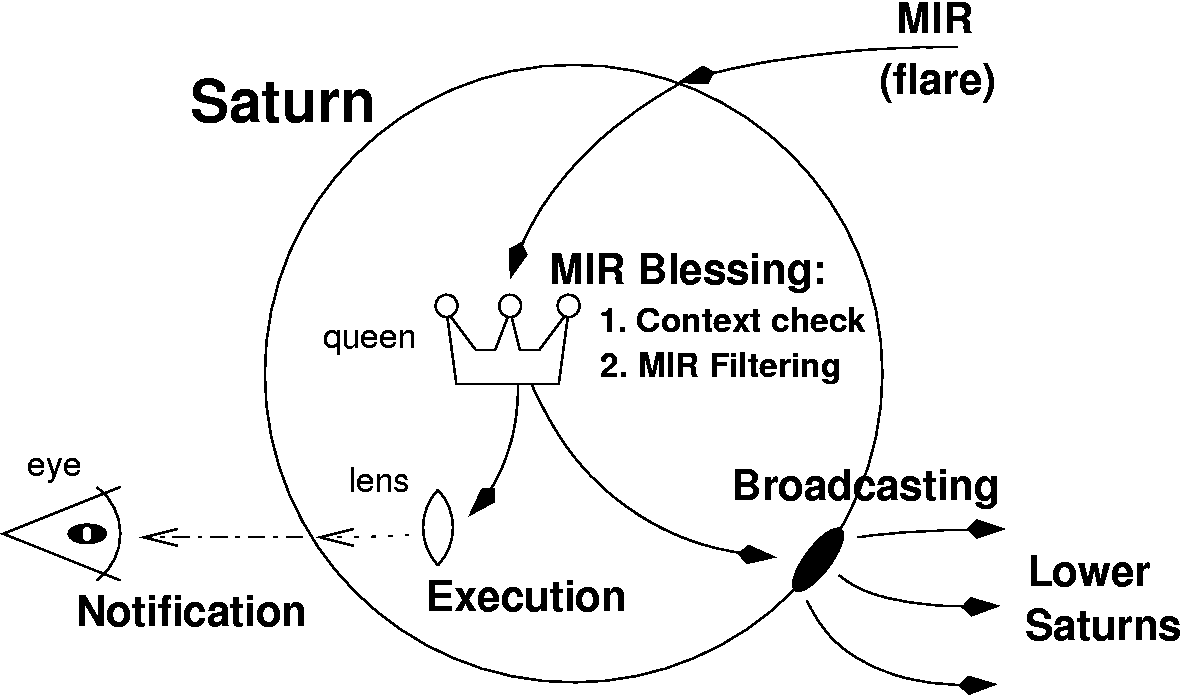
\includegraphics[width=7.2cm]{figs/flare_exec}
  \caption{Execution of a \emph{flare} on a Saturn. In case of a
    \emph{beam} the broadcasting of MIR is not performed.}
  \label{fig:flare_exec}
\end{figure}


\subsection{MIR Processing Performance Measurements}
%%%%%%%%%%%%%%%%%%%%%%%%%%%%%%%%%%%%%%%%%%%%%%%%%%%%%%%%%%%%%%%%%%%%%%%%
\label{ssec:DM_perf}

To benchmark the performance of the MIR processing mechanisms several
simple tests have been performed. The goal was to determine the
performance of the infrastructure itself and none of the tests does
anything useful: they simply invoke the relevant mechanisms of \gled.

The benchmarking code was implemented within the \gled framework
itself. The tests used thread execution environment of \gled
(described in more detail in Sec.\,\ref{sec:threads}) The execution
performance of an empty thread loop is shown in \emph{``Thread Loops''}
column of Tab.\,\ref{tab:MIRperf}.

Methods invoked in a context of a Saturn can optionally emit viewer
update requests or \emph{stamps} (see Sec.\,\ref{ssec:DM_Stamping}). As
stamping presents an execution penalty (serialization of the stamp,
broadcasting to viewers and processing of the stamp by viewers) the
two modes have been tested separately. In Tab.\,\ref{tab:MIRperf} they
are represented by column groups (a) \emph{``Method call''} (thread
calls an empty method in a lens) and (b) \emph{``Method call \&
  Stamp''} (the method also performs stamping). Furthermore, as
streaming and emitting of the stamp does not occur unless viewers are
connected to a Saturn, we have made two sets of measurements on each
machine: one with pure server and another with a single connected
viewer. For pure servers there is a minimal performance penalty
associated with stamping. In case (b) it is interesting to note the
performance benefits of a two-processor machine where server and
viewer threads can run in parallel.

For both methods types three different modes of method invocation have
been tested:
\begin{enumerate}
  
\item \textbf{Direct:} A direct method call. For empty method calls
  the cost is equvalent to the cost of a function call, while for
  methods with stamping the stamping procedure is also performed (note
  the drastic performance drop when a viewer is connected). These
  measurements also represent reference values for MIR-based
  invocation schemes described below.
  
\item \textbf{MIR:} MIR is created within the main thread and
  posted directly to the Saturn for processing and execution. All
  MIR processing proceeds within the same thread.
  
\item \textbf{Beamed MIR:} MIR is created on a client machine and sent
  to the server in \emph{beam} mode. Saturn's thread listening to client
  sockets receives the MIR, unpacks it and processes it as in the
  above case.
  
  It is important to note that the limiting factor was the processing
  speed of the server and not the available network bandwidth.

\end{enumerate}

\begin{table}[htbp]
  \def\valerr#1#2{#1}
  \small
  \centering
  \input perf.texf
  \smallskip
  \caption{Results of execution performance measurements for different
    machine configurations expressed in thousands of executions per second.
    AMD stands for \emph{AMD Athlon} and P3 for \emph{Pentium III}
    processor. See Sec.\,\ref{ssec:DM_perf}.
    }
  \label{tab:MIRperf}
\end{table}

The presented results show the execution penalties for different
elements of the \gled infrastructure. It is interesting to observe
that the measured performance spawns over one order of magnitude. In
real-life uses of \gled the very basic mechanisms would be used for
data transport and only a few specialized objects would emit viewer
update requests. By allowing a programmer to use an arbitrary
combination of framework elements, \gled can serve to implement a wide
range of advanced RPC techniques with optional continuous updating of
connected viewers. But as we have demonstrated that comes at a cost.

%%%%%%%%%%%%%%%%%%%%%%%%%%%%%%%%%%%%%%%%%%%%%%%%%%%%%%%%%%%%%%%%%%%%%%%%
%%%%%%%%%%%%%%%%%%%%%%%%%%%%%%%%%%%%%%%%%%%%%%%%%%%%%%%%%%%%%%%%%%%%%%%%

\section{Management of Saturn's Object-Spaces}
%%%%%%%%%%%%%%%%%%%%%%%%%%%%%%%%%%%%%%%%%%%%%%%%%%%%%%%%%%%%%%%%%%%%%%%%
\label{sec:saturn_os_management}

A sun-space and a fire-space of each Saturn are both managed (or
\emph{ruled}) by its \emph{king} lens. A king has purely
administrative duties: it holds its reserved object-space and
delegates \emph{queens} to actually rule upon their entrusted ID-space
chunks (\emph{queen-spaces}). Queens can be serialized to, or
resurrected from, comets (see Sec.\,\ref{ssec:dm_dmlam}) and they are
the smallest object-space elements that can be mirrored by lower
Saturns.

Upon connection, a new Saturn only receives serialized kings and
queens without the actual contents of their object spaces. The
mirroring of each queen-space is performed separately and can be
dynamically controlled. Request for mirroring of a queen on a given
Saturn (this request is also a MIR) can originate from any of the
Saturns that know about the existence of a given queen. A queen can be
marked as \emph{mandatory}: in this case all new Saturns are requested
to pull it into its moon-space.

Further, queens provide lens instantiation facilities: a lens can be
created and attached into the existing lens-graph by sending the queen
a single MIR. Lenses can be created as default objects (by sending
library set and class IDs of desired glass) or from an existing
serialized lens.

Another very important role of queens is \emph{blessing} of MIRs
directed at their subjects. A Saturn performs rudimentary context
checking to provide error trapping, while queens can offer extensive
dependency and access
control.\footnote{%
  The basic queen implementation of MIR blessing checks that all
  context arguments belong to the queen or to its dependencies. As all
  arguments of link and list modifications enter into the context part
  of a MIR, the consistency of object-spaces with respect to
  dependencies is guaranteed.} %
By sub-classing the \smalltt{ZQueen} class, a programmer can gain a
complete control over creation of lenses and their access in
respective queen-spaces.

Kings and queens are \emph{lenses} and they are placed in the first
available address of the ID object-space they are ruling. Each
\emph{ruler} also manages itself and can be accessed using the
standard \gled mechanisms (MIRs, GUI control).

A queen can depend on other queens in the same sun-space or in the
moon-space of a given Saturn. When a queen ${\cal Q}$ depends on a
queen ${\cal Q}'$, subjects of ${\cal Q}$ can reference subjects of
${\cal Q}'$ by either aggregation method (link to them or hold them as
list members). This means that ${\cal Q}'$ must be mirrored by a
Saturn prior to mirroring of ${\cal Q}$.  Otherwise the reconstruction
of ${\cal Q}$'s queen-space would result in unresolved references.

Queens can migrate to other kings, either to higher or lower levels in
Saturn hierarchy. This is facilitated by the ability of queens to
create comets. Saving them to disk, for permanent storage or swapping
purposes, is thus also possible.

\emph{Queen Types:}\ \ 
%%%%%%%%%%%%%%%%%%%
Ordinary queens are created with no subjects and later instantiate
them into their queen-spaces. When a lower level Saturn requests
mirroring of a queen-space, it has to be serialized and sent to the
moon. This is reasonable for dynamic data that is constantly changing.
But often one needs a static library of lenses that can be
referenced from other dependent queens. One such service is provided
by the \smalltt{IceQueen} class. Ice queens are instantiated from a
comet and block all incoming MIRs. Lower Saturns can instantiate them
in the same manner, by loading the comets from a permanent media, thus
saving the network bandwidth. Another option, semi-statical in
nature, is given by the \smalltt{FileQueen} class. File queens are
spawned over a ROOT file and provide a mapping from a full pathname to
a lens identifier. When sending such queens to a moon it is enough to
stream this mapping and the moon can instantiate the objects from the
local storage devices. A similar concept could be used for
connecting \gled's object-spaces to a database system.


\section{Representation and Management of a \gled Cluster}
%%%%%%%%%%%%%%%%%%%%%%%%%%%%%%%%%%%%%%%%%%%%%%%%%%%%%%%%%%%%%%%%%%%%%%%%

A \gled cluster is composed of Saturns organized in a tree structure.
Inside \gled each Saturn is represented by a lens of glass
\smalltt{SaturnInfo}. It provides the network identity of a given node
and is also the natural place to store access privileges and other
static or dynamic properties of a node.\footnote{E.g.\ node
  architecture, amount of RAM, CPU speed, load averages and other
  monitoring data.  Fig.\,\ref{fig:full_view} shows all GUI enabled data
  members of the \smalltt{SaturnInfo} glass.}  Further,
\smalltt{SaturnInfo} has three links: one to its master Saturn (for
SunAbsolute this is link is \smalltt{null}) and two to lists holding
its direct client Saturns and connected Eyes (viewers). Representants
of all Saturns are instantiated and maintained under a special queen,
called the \emph{sun-queen}. It is the first queen of the sun-king of
Sun Absolute and is pushed down to all connecting Saturns. This means
thateach node in a \gled cluster is always aware of the whole cluster
structure. Furthermore, this structure is rooted in the object-space
itself and directly accessible using the standard mechanisms of the
\gled paradigm.

A Saturn can accept connections from any number of Eyes. They also
have a corresponding \smalltt{EyeInfo} structure allowing each viewer
to have its own access privileges. Various messages can be sent
directly to an Eye, thus providing an efficient way for delivery of
messages, warnings and errors resulting from execution of MIRs
originating from the Eye in question.

Structure of a \gled cluster is therefore exported to all Saturns but
is managed centrally at the Sun Absolute. Any lens can get information
about any Saturn or Eye in the cluster and send it requests or
messages. A direct bridge can be opened between any two Saturns to
allow for node-to-node data transmissions.

The \smalltt{SaturnInfo} structure also holds unique identifications of
both sun-king and fire-king of its Saturn. By combining these IDs with
MIRs directed at the Saturn in question, kings can create queens in
their object-spaces on request from any Saturn in the cluster
(although the requesting Saturn might not be able to \emph{see} this
queen). These queens can then perform some computation on behalf of the
caller, either locally or by spreading it further down to lower level
Saturns.

In a similar manner connections between several \gled clusters could be
implemented.


%%%%%%%%%%%%%%%%%%%%%%%%%%%%%%%%%%%%%%%%%%%%%%%%%%%%%%%%%%%%%%%%%%%%%%%%
\section{Operators \& Threads}
%%%%%%%%%%%%%%%%%%%%%%%%%%%%%%%%%%%%%%%%%%%%%%%%%%%%%%%%%%%%%%%%%%%%%%%%
\label{sec:threads}

Each Saturn can run many threads simultaneously. A glass that needs to
acquire its own thread for a certain task or computation must be
sub-classed from the \smalltt{Eventor} glass. The common base provides
mechanisms for thread control and identification. Each
\smalltt{Eventor} contains a directory-like structure of
\smalltt{Operators} (also glasses) representing the actual algorithmic
elements of a thread. The operators can be traversed once or
several times until some exit condition is met. All thread operations
are therefore encapsulated in the framework and can be controlled with
MIRs as well as from \gled GUI.

Execution of and descending into individual operators can be
controlled at run-time, so the operator graph traversal is determined
by the state of its elements. Thread methods are exception throwing to
provide error recovery and thread state management facilities.

When a thread is created, its owner becomes the sender of the MIR that
triggered thread's execution. This is rather important as threads can
create MIRs and post them directly into a Saturn's routing system.
By accessing this information the Saturn can determine the owner of
the thread and set the caller ID of MIR accordingly.

Any method can be called from a thread (there is no built-in
restriction mechanism) and it is rather easy to spoil the consistency
of object-spaces by direct modification of lenses when a MIR should have
been used. Also, locks must be used when accessing data of lenses
which are not guaranteed to remain constant. Threads are no toys: they
are high-speed execution agents that would, if limited in their
execution power, hinder the computational performance of \gled.

Threads can be used to perform computations, certain periodical tasks
(such as monitoring of the node activity) or can be input-driven if
they perform I/O operations. They can also spawn new processes and act
as their supervisors, faithfully representing their state and
monitoring the output.


%%%%%%%%%%%%%%%%%%%%%%%%%%%%%%%%%%%%%%%%%%%%%%%%%%%%%%%%%%%%%%%%%%%%%%%%
\section{Viewing \& Rendering Infrastructure}
%%%%%%%%%%%%%%%%%%%%%%%%%%%%%%%%%%%%%%%%%%%%%%%%%%%%%%%%%%%%%%%%%%%%%%%%

GUI elements provided by an application framework/toolkit should be
general enough to allow implementation of a wide range of user
interfaces.  \gled GUI, as the rest of the system, is based on the
notion of extended \smalltt{C++} class: its main purpose is to allow
users to manipulate object-data and to invoke object-methods. This
implies that the application front-end has to be representable by a
collection of classes that hold the relevant configuration data and
implement the desired functionality.\footnote{In OO applications this
  is always the case, anyway.}  As a default GUI is provided for all
classes the prototype application GUI is readily available.

The GUI architecture is modular and extensible. Each library set can,
besides the auto-generated widgets for glasses, define their own GUI
elements. This, in principle, allows for construction of custom,
hand-made GUI front-ends and restricted user interfaces.

\subsection{Standard GUI elements}
%%%%%%%%%%%%%%%%%%%%%%%%%%%%%%%%%%%

Viewing objects are completely decoupled from the core of the \gled
system. They are managed by the \smalltt{Eye} class which serves as a
router between the local Saturn and actual viewing elements. Towards
the Saturn it transmits MIRs generated by lens-views in their GUI
callback functions. From Saturn it receives change notifications
objects (or \smalltt{Rays}) containing, among other things, the lens
identity and type of change that occurred (change of member data, links,
list contents, etc.). As each Eye holds a mapping from viewed
lenses to list of their lens-views, it can efficiently update all
views of the changed lens. This also implies that each lens can have
an arbitrary number of GUI representations.

The base class for lens-views (\smalltt{A\_View}) contains a minimal
representation of the observed lens and some abstract methods for handling
of change notifications. Further base classes are provided for
representations of links and lists.
%
Automatically generated widgets for lenses as well as the hand-made GUI
front-end are all built upon these base classes. As details of the
implementation are beyond the scope of this article, the emphasis will
be put on features of the GUI (implemented using the \smalltt{FLTK}
widget library \cite{fltk}).

% full view
For each lens a window containing a collection of all automatically
generated widgets for a given lens can be created (e.g.\ 
Fig.\,\ref{fig:full_view}). It includes widgets for all parent
classes, ordered by the class hierarchy.

\begin{figure}
  \centering
  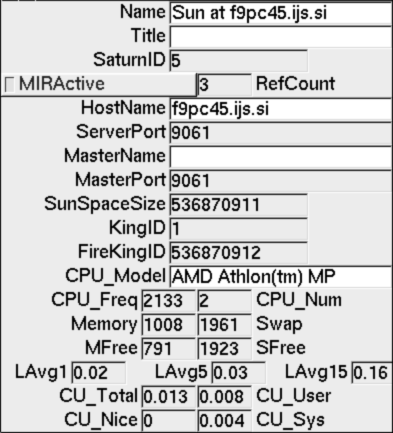
\includegraphics[width=4.5cm]{figs/full_view}
  \caption{A \emph{full-lens-view} for the \foottt{SaturnInfo} glass.}
  \label{fig:full_view}
\end{figure}

% lens browser
An important feature of the \gled GUI is a generalized structure
browser (\emph{lens-browser}). It displays lenses together with their
list members and links. The list members are shown in a collapsible
vertical structure (as in most standard file/object browsers) while
links are represented in a horizontal structure, allowing more compact
views of selected lenses (e.g.\ Fig.\,\ref{fig:link_view}). The
lens-browser provides a means for manipulation of links, modification
of list contents and instantiation of new lenses. Lenses can also be
exported into the C++ interpreter shell for manual operations.

\begin{figure*}
  \centering
  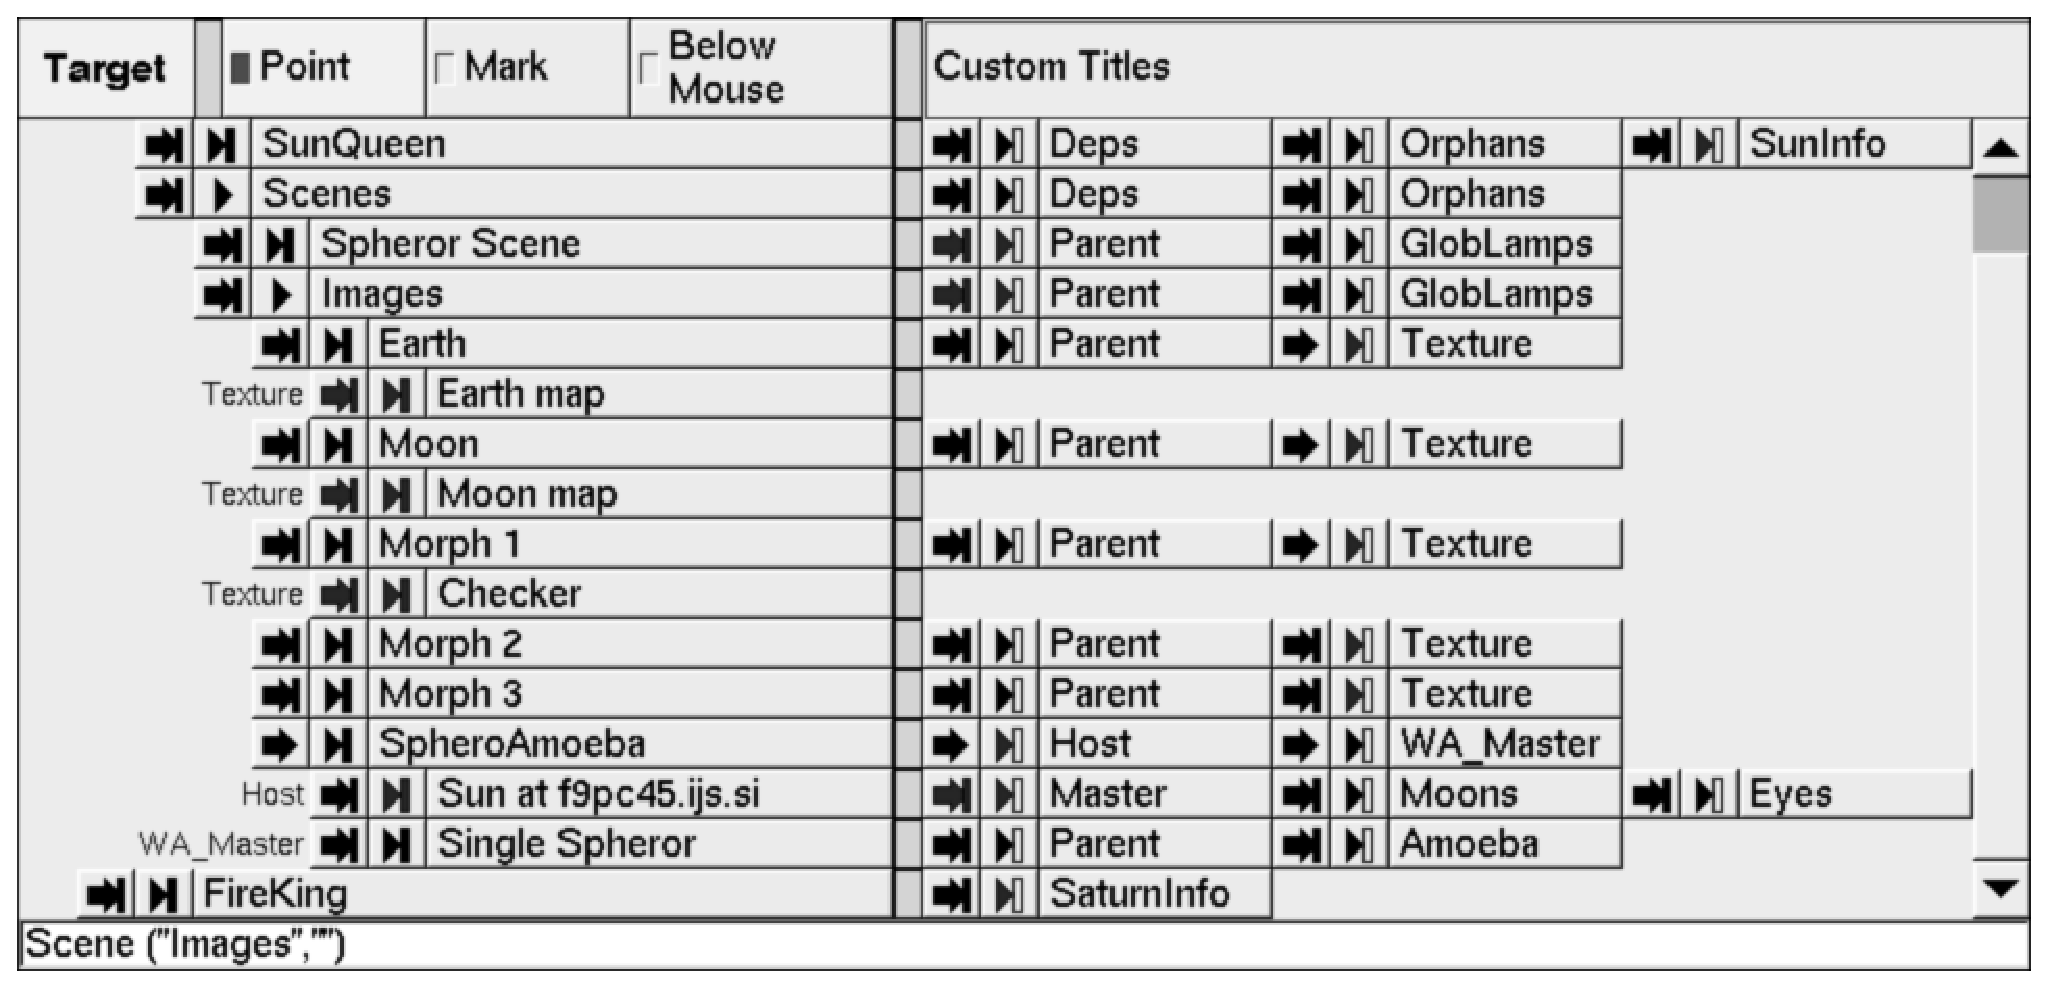
\includegraphics[width=0.86\textwidth]{figs/link_view}
  \caption{A lens browser displaying a lens graph. Each entry has two
    collapsing buttons: one for links and the other for list members.
    Links of each lens are displayed on the right part of the
    browser.}
  \label{fig:link_view}
\end{figure*}

The lens-browser has another mode in which its right part contains a
custom set of widgets for each lens (sub-selection of those from a
full-lens-view).  The desired glasses and their members can be
specified using a simple syntax.  A specialized parser then creates
the appropriate widgets for each lens (Fig.\,\ref{fig:custom_view}).
Such views provide an efficient way for viewing and editing of a large
number of lenses.

\begin{figure*}
  \centering
  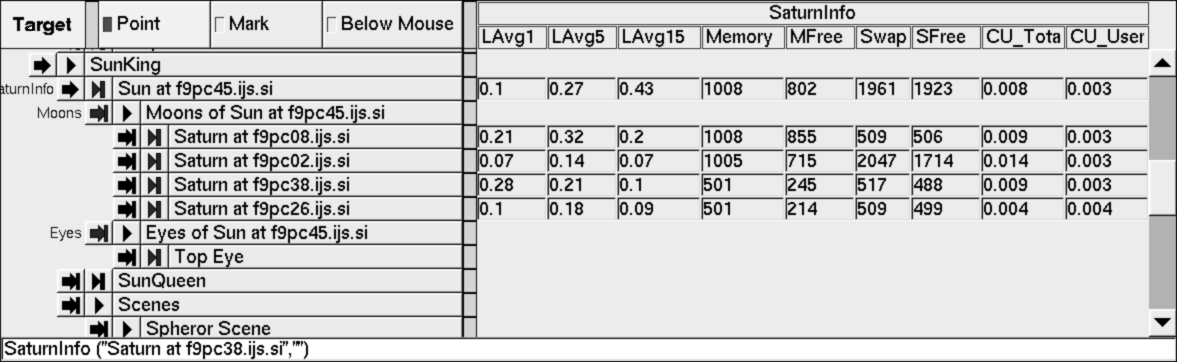
\includegraphics[width=\textwidth]{figs/custom_view}
  \caption{A set of custom-generated widgets inside a lens browser
    showing \foottt{SaturnInfo} structures for a \gled cluster
    composed of five nodes.}
  \label{fig:custom_view}
\end{figure*}


\subsection{Rendering}
%%%%%%%%%%%%%%%%%%%%%%

The rendering infrastructure offers the representation of lenses and
lens-graphs in 3D space. Actual rendering of lenses is done by a
parallel class structure that has to be coded manually for each
rendering device.\footnote{OpenGL is used as the standard real-time
  renderer, others can be added using a common render-driver API.}
It is not mandatory for glasses to have a corresponding rendering
class: they can use the renderer of any of their base classes.
Rendering classes for each device and each library set are produced as
independent libraries and can be dynamically loaded into a running
\gled system.

A high level of flexibility is achieved by actual rendering of each
lens being split into three functions: \smalltt{PreDraw()},
\smalltt{Draw()} and \smalltt{PostDraw()}. Further, rendering is
proceeding on an arbitrary number of levels allowing the draw methods
of the lens, its links and list members to be called in any order.
This provides a versatile infrastructure for traversal of lens-graphs
as well as for management of renderer state (lighting, polygon mode,
material properties, texturing, etc.).

More examples of \gled's GUI and can be found at the
project's homepage\cite{gled.org}.

%%%%%%%%%%%%%%%%%%%%%%%%%%%%%%%%%%%%%%%%%%%%%%%%%%%%%%%%%%%%%%%%%%%%%%%%
\section{Applications of the \gled system}
%%%%%%%%%%%%%%%%%%%%%%%%%%%%%%%%%%%%%%%%%%%%%%%%%%%%%%%%%%%%%%%%%%%%%%%%

We have presented the core functionality of the \gled system which,
from this perspective, offers an OO framework. However, if one is
interested in building a distributed application, the base classes of
\gled can be seen as elements of a toolkit. Future work will, among
other things, focus on development of library sets (offering
particular implementations for selected areas of interest) and
preparation of corresponding demonstration programs. Based on these,
\gled will also become a toolkit for respective development areas.

To conclude this paper the \gled system will be discussed from the point
of view of four different usage modes. This will serve to recapitulate
the main ideas, to merge the presented details into a coherent whole
and to discuss future extensions of \gled.

\subsection{Single machine, single user usage}
%%%%%%%%%%%%%%%%%%%%%%%%%%%%%%%%%%%%%%%%%%%%%%

\gled classes can serve as an interface to configuration and execution
of user algorithms as well as for visualization of resulting data.
Persistency of configuration data and results of algorithms is
achieved by using ROOT's object serialization and I/O infrastructure
(ROOT files and trees).

Glass member functions can hold the implementation of the algorithms or
can serve as a wrapper layer for a specialized (numerical) library
which can be implemented in any language linkable with \smalltt{C++}.
By sub-classing the base thread glass (\smalltt{Eventor}) finer
control over operation and configuration of algorithms can be
achieved.

As GUI classes are automatically generated for all glasses, they can
immediately serve for composition of object graphs, for configuration
and editing of member data and for algorithm control via management of
threads. CINT, the \smalltt{C/C++} interpreter, offers a general
scripting interface to all \gled's functionality and thus
complements the GUI functionality for complex and repetitive tasks.

Standard data presentation services, such as histograms and graphs,
are offered by the ROOT system. Further, ROOT has a rich set of tools
and algorithms for statistical analysis, minimization and spectral
analysis.

Dynamic real-time 3D visualization can easily be programmed by
providing the rendering classes and using the \smalltt{Eventor}-thread
infrastructure. As rendering crucially depends on the underlying
data-structures it is hard, if not impossible, to provide a generic
and efficient set of rendering atoms. However, for some specific cases
the renderers are already available. E.g.\ a representation of a 2D
function on a rectangular mesh (using ROOT's \smalltt{TMatrix} class)
and 3D triangulated surfaces (wrapper over GTS library \cite{gts}).
Further rendering elements will become available with appearance of
new library sets and with their proper structuring \gled will offer a
generic multi-purpose rendering toolkit.

\subsection{Distributed and \grid computing}
%%%%%%%%%%%%%%%%%%%%%%%%%%%%%%%%%%%%%%%%%%%%

The \gled framework enables prototyping and control of algorithms
performing computation or dynamic visualization within a hierarchic
server-client-viewer model. As topology of the cluster is not limited
and can also change dynamically, sophisticated problem solving
strategies can be implemented over heterogenous clusters (MIRs and
streamed data are architecture independent).

A particularly interesting feature of \gled is that the cluster
structure itself is directly accessible to algorithms using the
standard framework mechanisms. On one hand this provides a means for
cluster monitoring and visualization while on the other it allows for
dynamic optimization of the cluster structure.

Currently there are no central mechanisms for node allocation and
acquisition. Such mechanisms will be implemented as daemons or network
services with a top-level node manager. Another option is to adopt \grid
resource allocation services when they become standardized. Until then
standard remote command execution mechanisms can be used (e.g.\ 
\smalltt{rsh} or \smalltt{ssh}).

Each node in a distributed cluster and each thread within a node
analyses and/or produces data. Based on the nature of the problem,
different solutions for emitting the resulting data may be applied.
\begin{itemize}
\item If the data is segmented into many relatively small fragments or
  is needed for continuation of computation on some other node, then
  it can be sent encapsulated into a MIR. The object that
  receives the MIR can properly place the data into a larger structure or
  further propagate it to relevant algorithms. Arguments of the MIR
  can serve as instructions for management of the subsequent data.
  This way MIRs can serve as carriers for a sophisticated data
  exchange protocol.
\item If the data is produced in large fragments and is not
  instantly needed for further computation then it can be emitted via
  standard data-exchange mechanisms, e.g.\  \smalltt{ftp},
  \smalltt{rootd} (remote access to ROOT files) or distributed
  file-systems (nfs, afs). The data can also be cached in the vicinity
  of the local node and transmitted on request upon completion of the
  computation on a larger scale. This allows minimal network
  connection duration and provides means for shaping of the network
  traffic.
\end{itemize}
Similar problems arise when algorithms need read access to shared
data. Further development of \gled will also address various data
exchange mechanisms and will offer some concrete implementations of
data traffic structuring and \grid-aware data addressing protocols.

\subsection{Multi-user information systems}
%%%%%%%%%%%%%%%%%%%%%%%%%%%%%%%%%%%%%%%%%%%

Hierarchic structure of the \gled cluster makes it an interesting
platform for implementation of collaborative tools and VR systems.
Intermediate proxy nodes can provide an effective reduction of network
traffic when several nodes from several organizations are connected
into a common information system.

The concurrent access of several user requires an elaborate
authentication \& access control mechanism. Implementation of such
infrastructure is under way. Authorization is performed during MIR
processing stage (as a part of blessing of a MIR by a \smalltt{Queen})
and further infrastructure is being implemented that allows individual
lenses and \smalltt{Queens} to specify access policy. At first \gled
will use internal user and group databases and in due time interfaces
to appropriate LDAP and \grid services will be created.

As \gled offers a direct correspondence between lenses and their 3D
representations, advanced VR systems with immersive control over
object graphs can be implemented. This requires further work on UI
infrastructure, which has to provide mechanisms for creation of
complex object contexts with transparent access to available member
functions and their arguments. However, the infrastructure for
emitting MIRs from UI and receiving update requests is implemented as
a part of the core system. The available GUI elements
(full-lens-views, lens-browser and GL rendering window) provide a
general interface to mechanisms of the \gled system and offer an
example of complexity that can be achieved by indirect mapping of
lenses to GUI structures.

\subsection{Encapsulated network services}
%%%%%%%%%%%%%%%%%%%%%%%%%%%%%%%%%%%%%%%%%%

By encapsulating network services with\-in a sub-class of the
\smalltt{Eventor} glass, threads from within the Saturn can offer any
kind of service to outside clients, for example:
\begin{itemize}
\item Provide information about local Saturn and local computing node
  (status, monitoring data, catalog of locally available data and
  availability of other services).
\item Export its object-spaces and local data to consumers by using
  any desired protocol. For example, lens graphs and lens data could
  be exported via \smalltt{http} protocol in \smalltt{html} or
  \smalltt{xml} format.
\item Serve as entry point for computation or service instantiation
  requests. After a successful authentication such request can result
  in creation of a thread that will provide the required service.
\item Serve as entry point for data coming from external sources, such
  as other processes or sensors connected to the node.
\end{itemize}

In this respect \gled offers monitoring and replication facilities for
such services as well as infrastructure for following and reporting
the usage patterns (ROOT trees, histograms and graphs). It is also an
advantage that multiple services can be spawned from within the same
process: it allows for easier load balancing between different
services and allows implementation of advanced strategies for
resolving complex queries (e.g.\ \grid resource allocation requests) or
providing parallel file I/O operations.


%%%%%%%%%%%%%%%%%%%%%%%%%%%%%%%%%%%%%%%%%%%%%%%%%%%%%%%%%%%%%%%%%%%%%%%%
\section{Conclusion}
%%%%%%%%%%%%%%%%%%%%%%%%%%%%%%%%%%%%%%%%%%%%%%%%%%%%%%%%%%%%%%%%%%%%%%%%

The \gled system brings together a colorful collection of modern
computing techniques and binds them within a fairly general
implementation of a hierarchic server--client model. By merging
cluster creation and configuration tools, object-based RPC, threaded
exectuion environment, automatically generated GUI widgets and
sophisticated 3D rendering infrastructure, \gled has been shown to
represent a useful OO framework/toolkit for development of a number of
distinctly different applications that can take advantage of
distributed computing environment, object serialization, cooperative
multi-user GUI and rich data presentation \& visualization
infrastructure. In \gled these complex techniques are represented at a
fairly abstract level but at the same time a low-level interface is
available to allow for further extensions and more specialized
implementations.

We hope that \gled addresses the demands and possibilities of modern
computing in a fashion that is both interesting as a research project
and usable as a concrete framework implementation.


%%%%%%%%%%%%%%%%%%%%%%%%%%%%%%%%%%%%%%%%%%%%%%%%%%%%%%%%%%%%%%%%%%%%%%%%
\section*{Availability}
%%%%%%%%%%%%%%%%%%%%%%%%%%%%%%%%%%%%%%%%%%%%%%%%%%%%%%%%%%%%%%%%%%%%%%%%

The implementation of the described framework is publicly available
\cite{gled.org}. While \gled is constantly developing, its core
functionality is stable and suitable for implementation of production
systems. As it is with any open-source project, the future
development of \gled largely depends on interests and contributions
from users of outside communities.

%%%%%%%%%%%%%%%%%%%%%%%%%%%%%%%%%%%%%%%%%%%%%%%%%%%%%%%%%%%%%%%%%%%%%%%%
\section*{Acknowledgments}
%%%%%%%%%%%%%%%%%%%%%%%%%%%%%%%%%%%%%%%%%%%%%%%%%%%%%%%%%%%%%%%%%%%%%%%%

I am infinitely indebted to my friend J.~J.~Javor\v{s}ek for his
support and enthusiasm for the \gled project. Without his
willingness to spend countless hours discussing the arising problems
and ideas \gled, most probably, would not exist at all.

Many thanks go to teams developing ROOT, \smalltt{perl}, \textsc{Fltk}
and GNU development tools for excellent packages that make the burdens
of software development bearable.

%%%%%%%%%%%%%%%%%%%%%%%%%%%%%%%%%%%%%%%%%%%%%%%%%%%%%%%%%%%%%%%%%%%%%%%%
% References
%%%%%%%%%%%%%%%%%%%%%%%%%%%%%%%%%%%%%%%%%%%%%%%%%%%%%%%%%%%%%%%%%%%%%%%%

\begin{thebibliography}{99}
  
\bibitem{root} R.~Brun and F.~Rademakers, \emph{ROOT -- An Object
    Oriented Data Analysis Framework}, Proceedings AIHENP'96 Workshop,
  Lausanne, Sep. 1996, Nucl. Inst. \& Meth. in Phys. Res. A 389 (1997)
  81-86. See also \url{http://root.cern.ch/}.
  
\bibitem{seti} SETI@home, \emph{The Search for Extraterrestrial
    Intelligence}, \url{http://setiathome.ssl.berkeley.edu/}.
  
\bibitem{folding} Folding@home, \emph{Distributed protein folding
    simulations}, \url{http://folding.stanford.edu/}.

\bibitem{rpc} A.D.~Birrell and B.J.~Nelson, \emph{Implementing Remote
    Procedure Calls}, XEROX CSL-83-7, October 1983.
      
\bibitem{xdr} R.~Srinivasan, \emph{XDR: External Data Representation
    Standard}, RFC 1832, Sun Microsystems, Inc., August 1995.
        
\bibitem{ldap} W.~Yeong, T.~Howes and S.~Kille, \emph{Lightweight
    Directory Access Protocol}, RFC 1777, Performance Systems
  International, University of Michigan, ISODE Consortium, March 1995.
  
\bibitem{cint} M.~Goto, \emph{C++ Interpreter - CINT}, CQ publishing,
  ISBN4-789-3085-3 (Japanese).

\bibitem{fltk} B.~Spitzak, et al, \emph{FLTK -- A Fast Light ToolKit},
  \url{http://www.fltk.org/}.
  
\bibitem{gled.org} The \gled project homepage: \url{http://www.gled.org/}.
  
\bibitem{gts} \emph{GTS -- GNU Triangulated Surface Library},
  \url{http://gts.sourceforge.net/}.

\end{thebibliography}

\end{document}

%%%%%%%%%%%%%%%%%%%%%%%%%%%%%%%%%%%%%%%%%%%%%%%%%%%%%%%%%%%%%%%%%%%%%%%%
%%%%%%%%%%%%%%%%%%%%%%%%%%%%%%%%%%%%%%%%%%%%%%%%%%%%%%%%%%%%%%%%%%%%%%%%

% LocalWords:  ftw accessor ROOT's forwards MIR's threadable Saturns MIRs API
% LocalWords:  RPC XDR LDAP
